\chapter{Modelli per la  gestione dei BES}
\label{cha:ModellogestioneBES}
%\begin{center}
%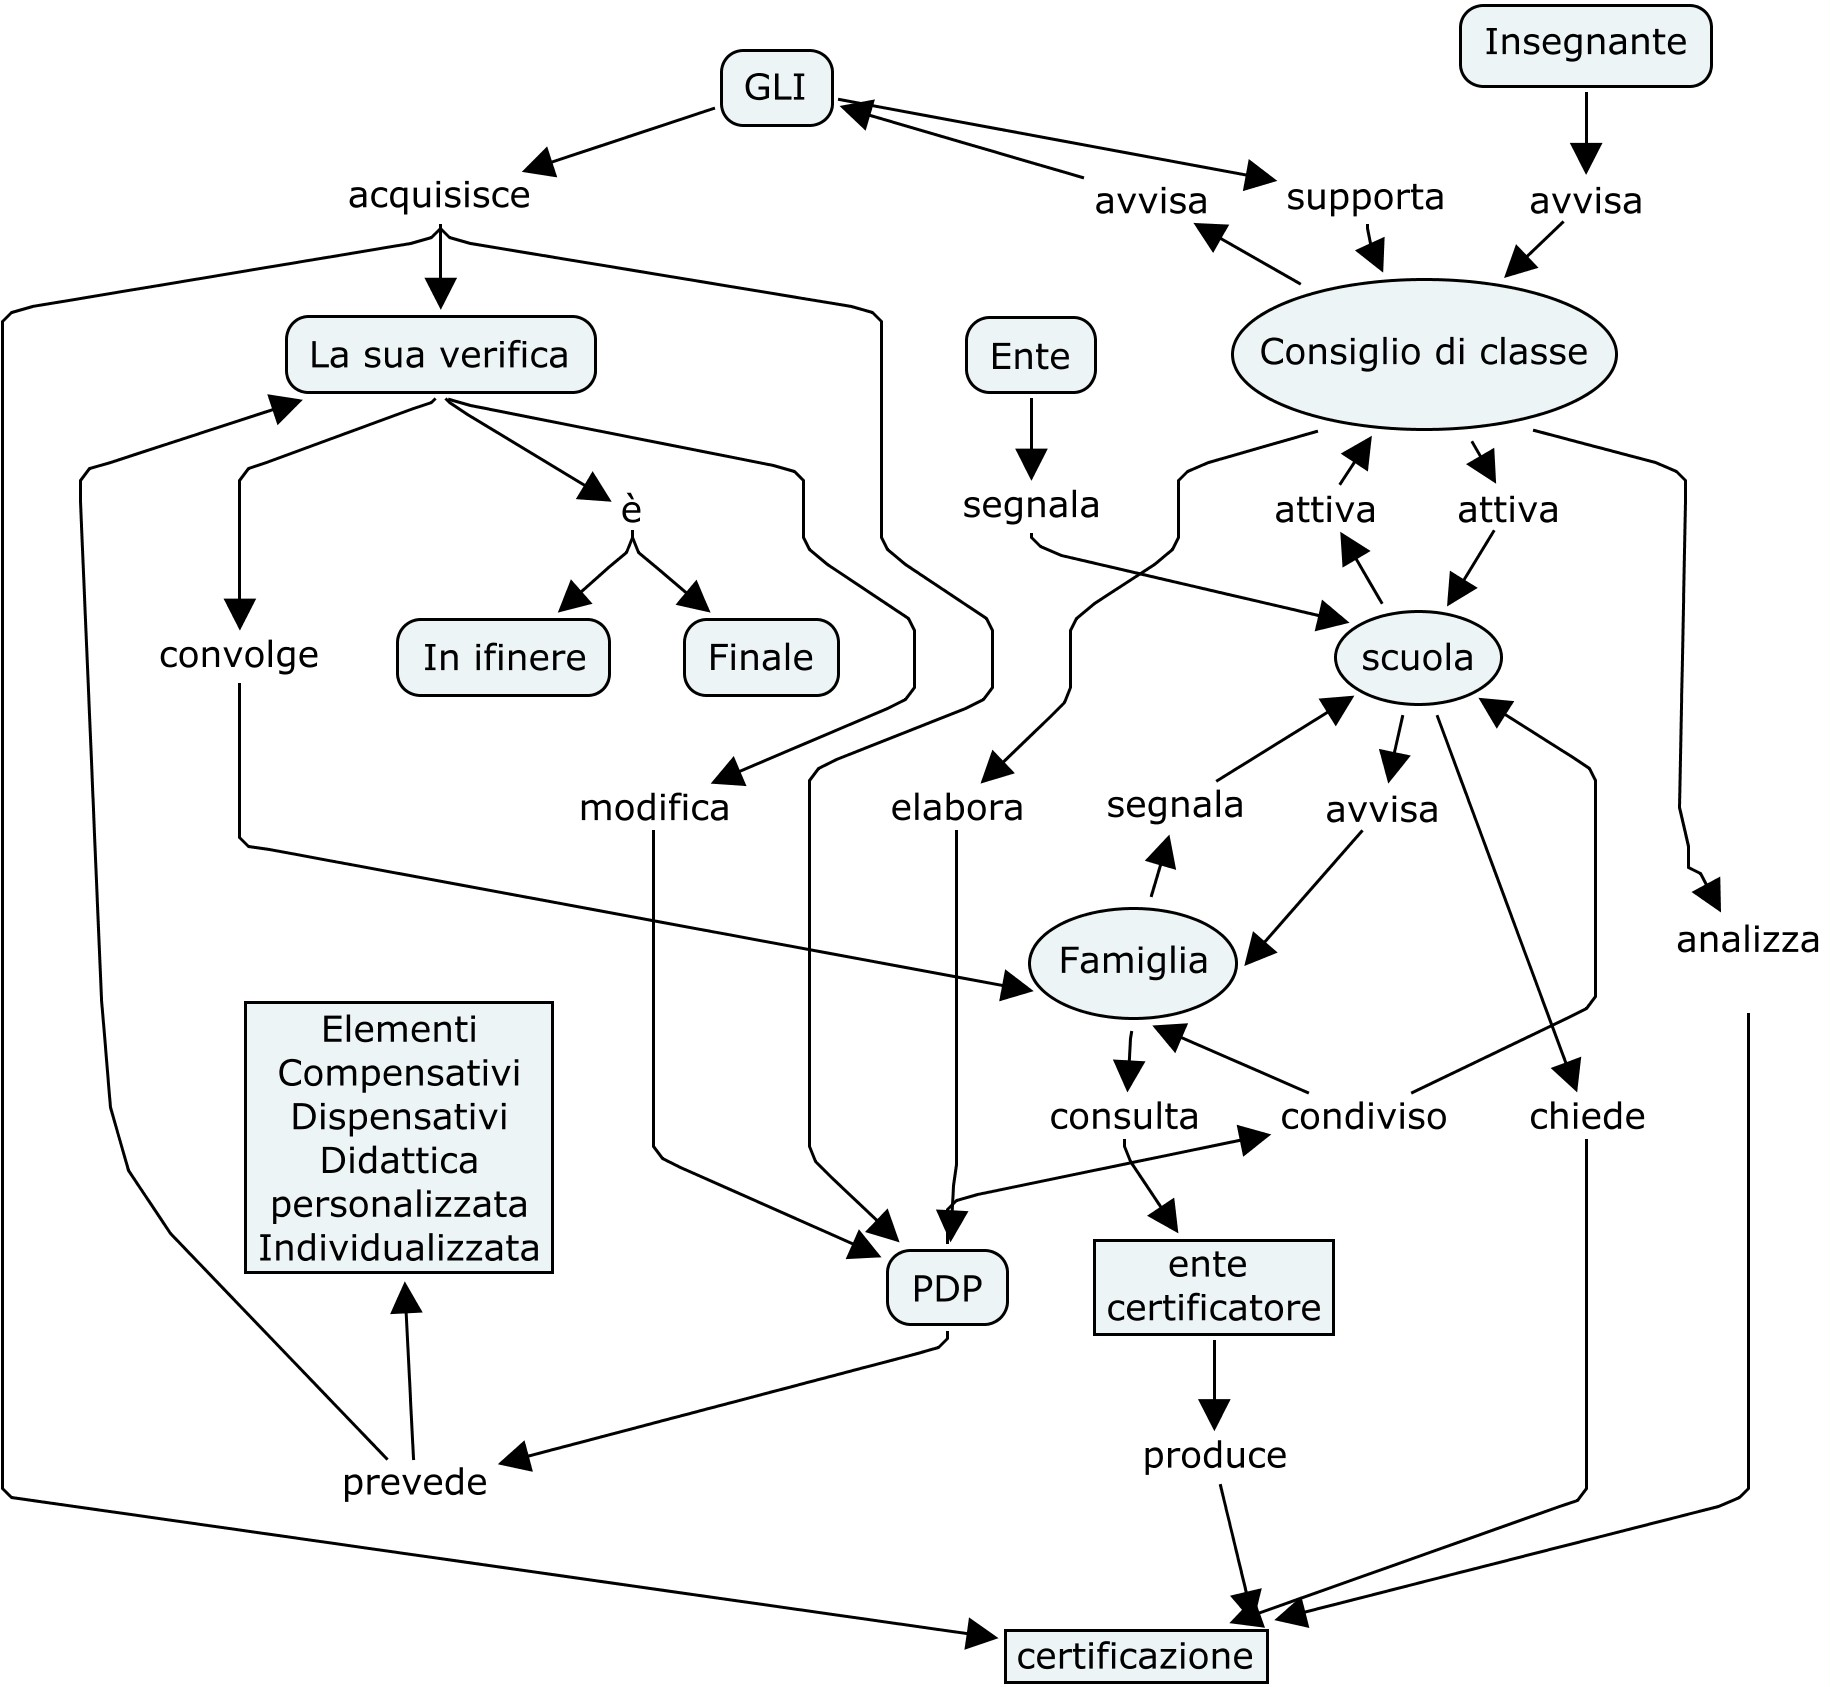
\includegraphics[scale=0.23]{bes3.jpg}
%\end{center}
Possiamo classificar i BES in tre gruppi, Lo schema\vref{fig:besschema} mostra a grandi linee cosa prevede la normativa. 
 \begin{figure}[t]
 	\centering
 	\includegraphics[width=1\linewidth, height=1\textheight]{bes schemab.pdf}
 	\caption[Classificazione]{Classificazione}
 	\label{fig:besschema}
 \end{figure}
La gestione degli alunni in BES è molto complessa. La procedura\vref{fig:bes3} che segue mostra come tre entità: la famiglia, la scuola, il Consiglio di Classe possono interagire per prendere in carica lo studente. Nella schema è presente anche il GLI, che ha funzioni di coordinamento, supporto e raccolta di informazioni. Lo schema dovrebbe essere condiviso con tutti in modo che ogni componente del sistema sa cosa deve fare. 
\begin{figure}[t]
\centering
\includegraphics[width=1\linewidth, height=1\textheight]{bes3c}
\caption[Gestione BES]{Proposta di gestione di un alunno con BES}
\label{fig:bes3}
\end{figure}



